% This text is proprietary.
% It's a part of presentation made by myself.
% It may not used commercial.
% The noncommercial use such as private and study is free
% Sep. 2005 
% Author: Sascha Frank 
% University Freiburg 
% www.informatik.uni-freiburg.de/~frank/


\documentclass{beamer}

\usepackage{graphicx}

\begin{document}
\title{Metasix}   
\author{Rafael Santana} 
\date{\today} 

\frame{\titlepage} 

%\frame{\frametitle{Table of contents}\tableofcontents} 

\section{Usando Branchs} 

\frame{ 
\begin{figure}[h!]
\centering
{\fontsize{1cm}{1em}\selectfont Usando \textit{Branchs}}
\end{figure}
}

\frame{\frametitle{Exemplo (parte 1)} 
\begin{figure}[h!]
\centering
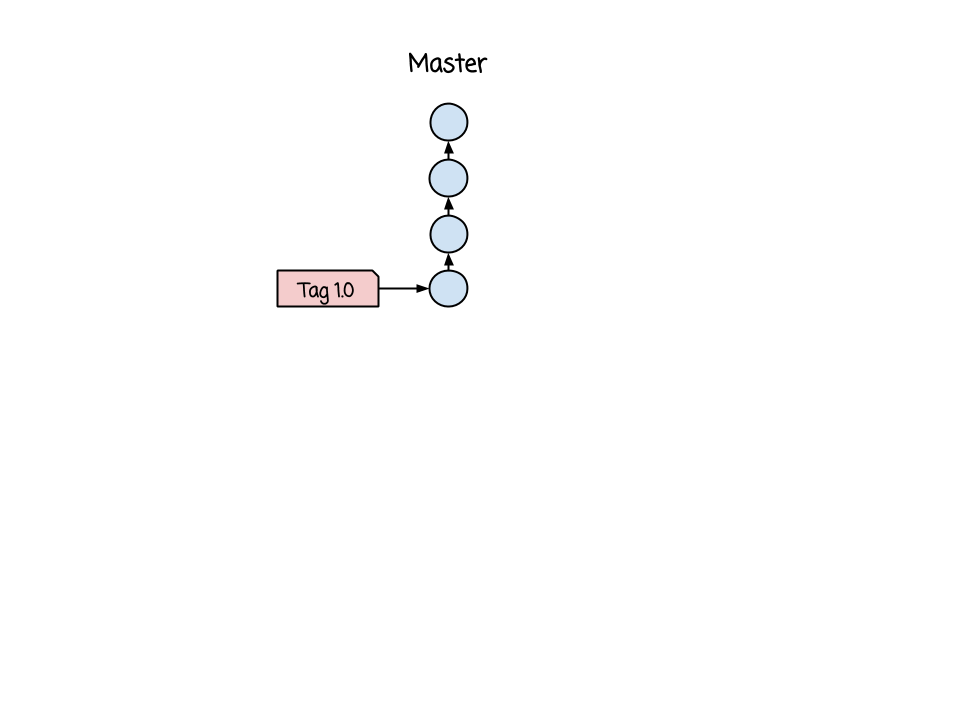
\includegraphics[width=1\textwidth]{img/exemplo-01}
\end{figure}
}

\frame{\frametitle{Exemplo (parte 2)} 
\begin{figure}[h!]
\centering
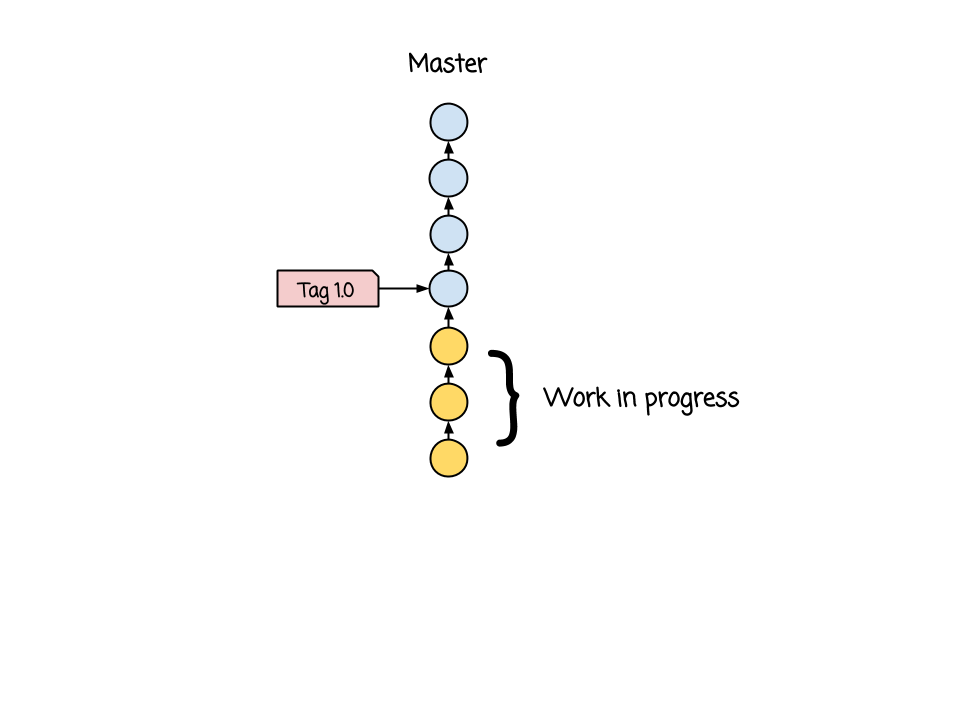
\includegraphics[width=1\textwidth]{img/exemplo-02}
\end{figure}
}

\frame{\frametitle{Exemplo (parte 3)} 
\begin{figure}[h!]
\centering
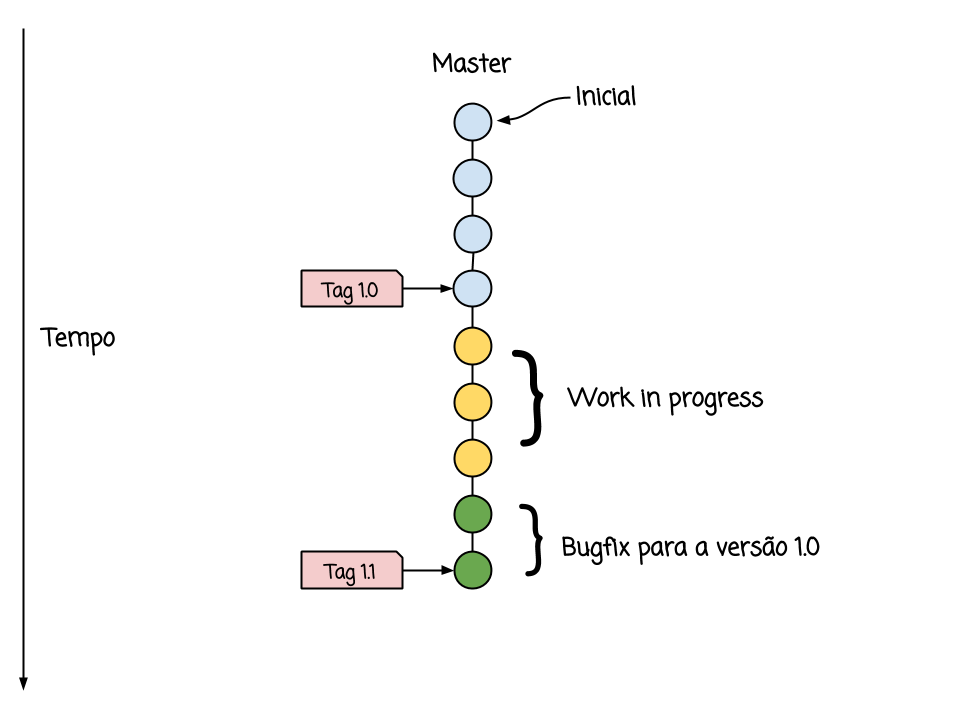
\includegraphics[width=1\textwidth]{img/exemplo-03}
\end{figure}
}

\frame{\frametitle{Exemplo (parte 4)} 
\begin{figure}[h!]
\centering
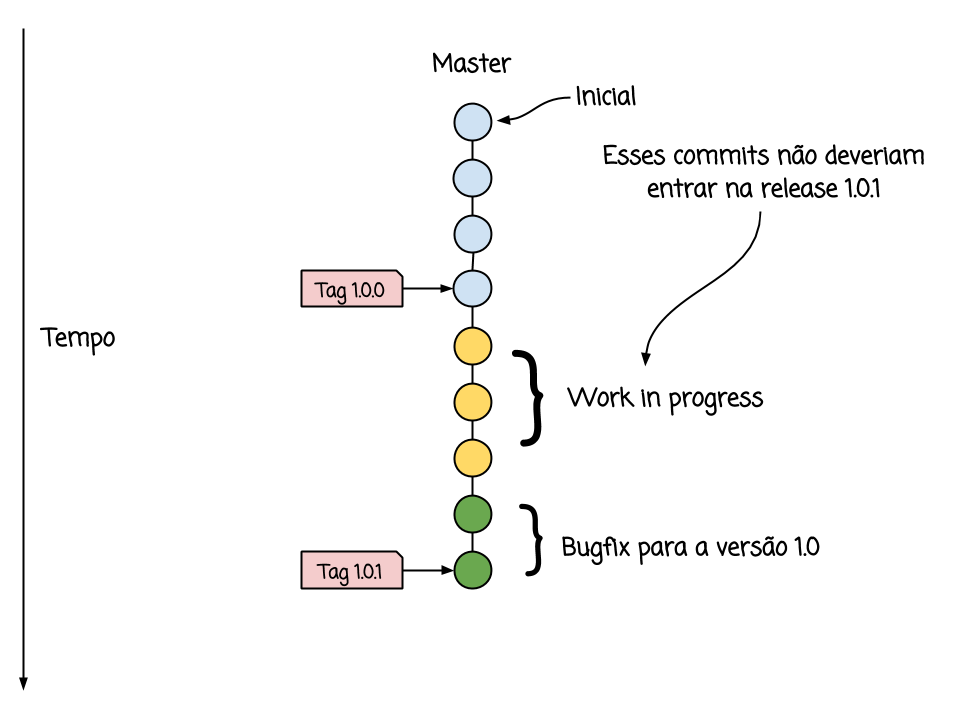
\includegraphics[width=1\textwidth]{img/exemplo-04}
\end{figure}
}

\frame{\frametitle{Exemplo (parte 5)} 
\begin{figure}[h!]
\centering
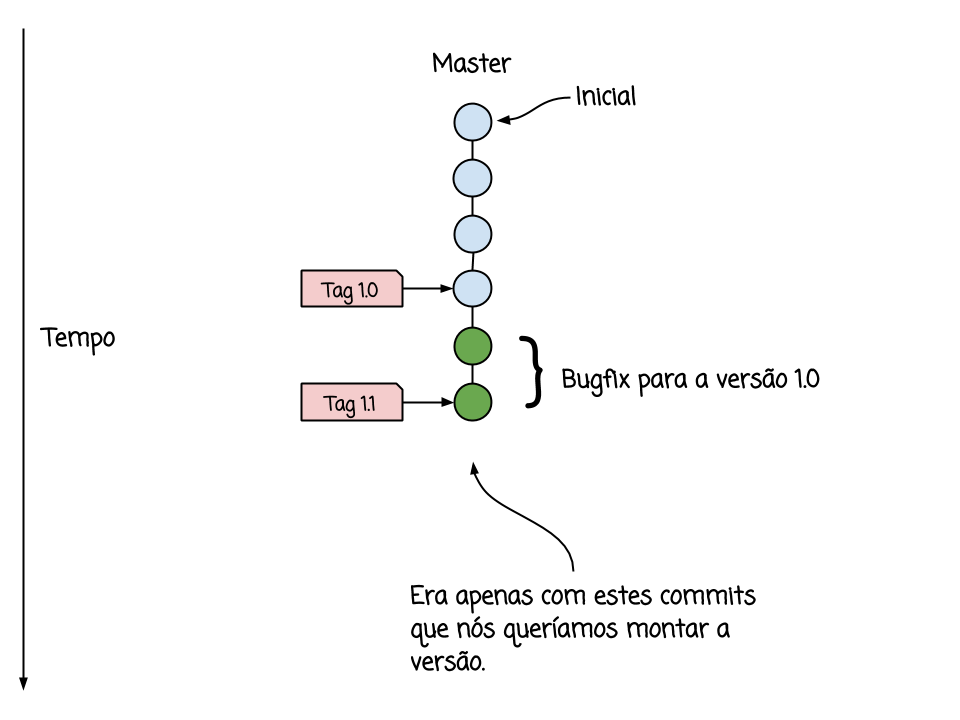
\includegraphics[width=1\textwidth]{img/exemplo-05}
\end{figure}
}

\frame{\frametitle{Boa Pratica (1)} 
\begin{figure}[h!]
\centering
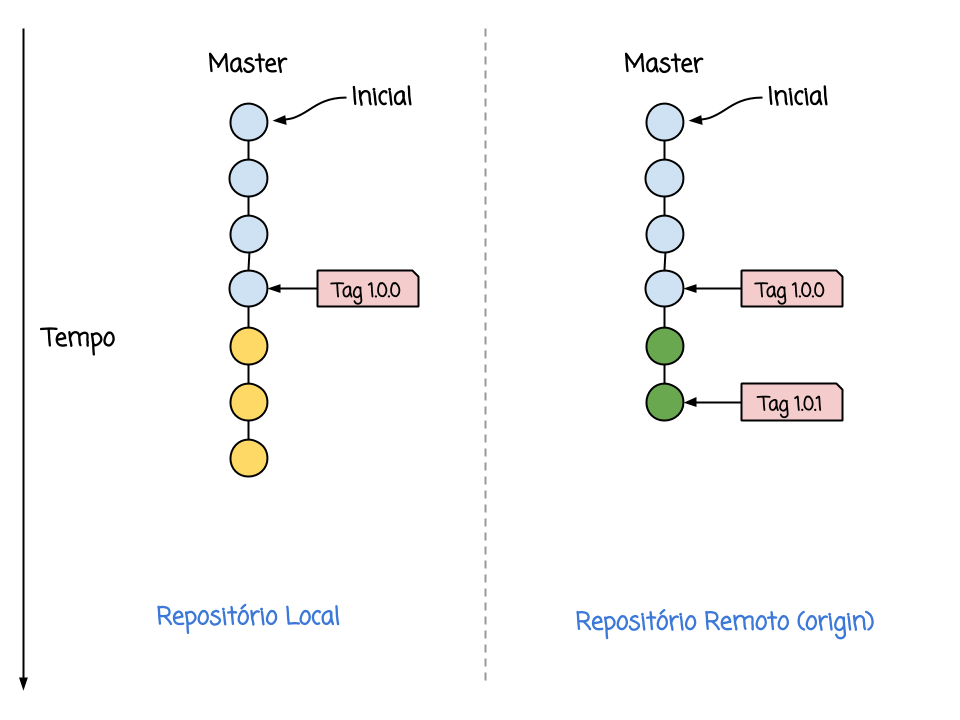
\includegraphics[width=1\textwidth]{img/solutions-01}
\end{figure}
}

\frame{\frametitle{Boa Pratica (2)} 
\begin{figure}[h!]
\centering
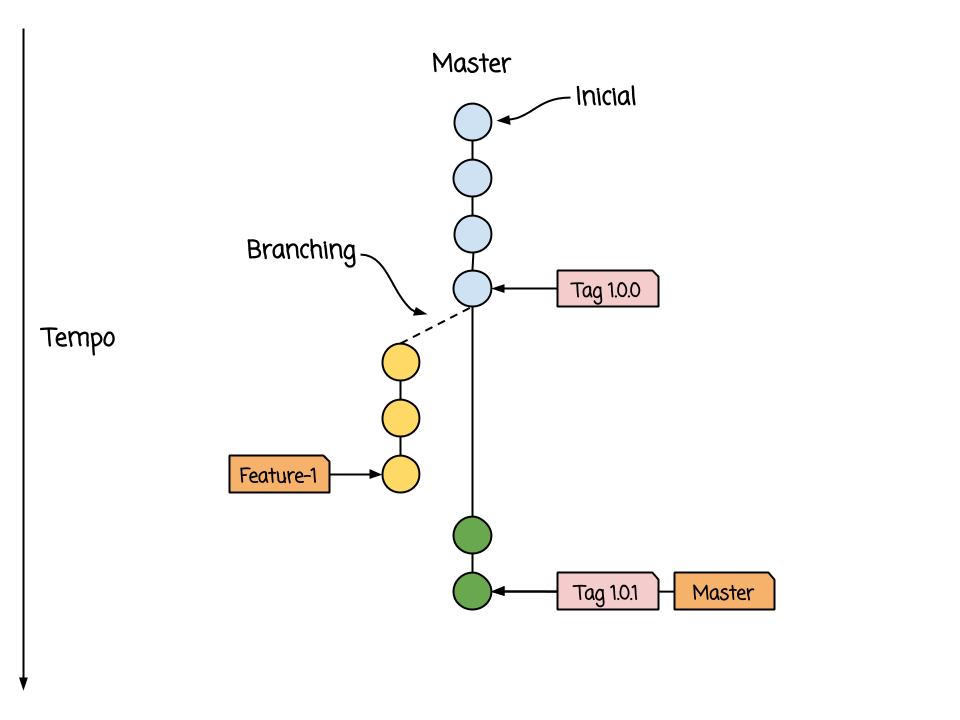
\includegraphics[width=1\textwidth]{img/solutions-02}
\end{figure}
}

\frame{\frametitle{Modelo para Uso de Branchs} 
    \begin{itemize}
        \item existem muitos modelos para uso de \textit{branchs};
        \newline
        \item suas vantagens ou desvantagens dependem da necessidade de cada equipe;
        \newline
        \item nossa rotina hoje nao exige um modelo complexo.
    \end{itemize}
}

\frame{\frametitle{Modelo para Uso de Branchs} 
    \textit{Branchs} permanentes
    \begin{itemize}
        \item \textbf{Master}: \textit{branch} principal; 
        \newline
    \end{itemize}
    \textit{Branchs} de apoio
    \begin{itemize}
        \item \textbf{Feature}: usadas durante o desenvolvimento de novas
            funcionalidades. (e.g, feature-142);
        \newline
        \item \textbf{Bug}: usadas para \textit{bugfixes}. (e.g, bug-13);
        \newline
        \item \textbf{Enhancement}: usadas para o desenvolvimento de melhorias
            do projeto. (e.g, enhancement-76).
    \end{itemize}
}

\frame{\frametitle{Proposta de Processo de Trabalho (parte 1)} 
\begin{figure}[h!]
\centering
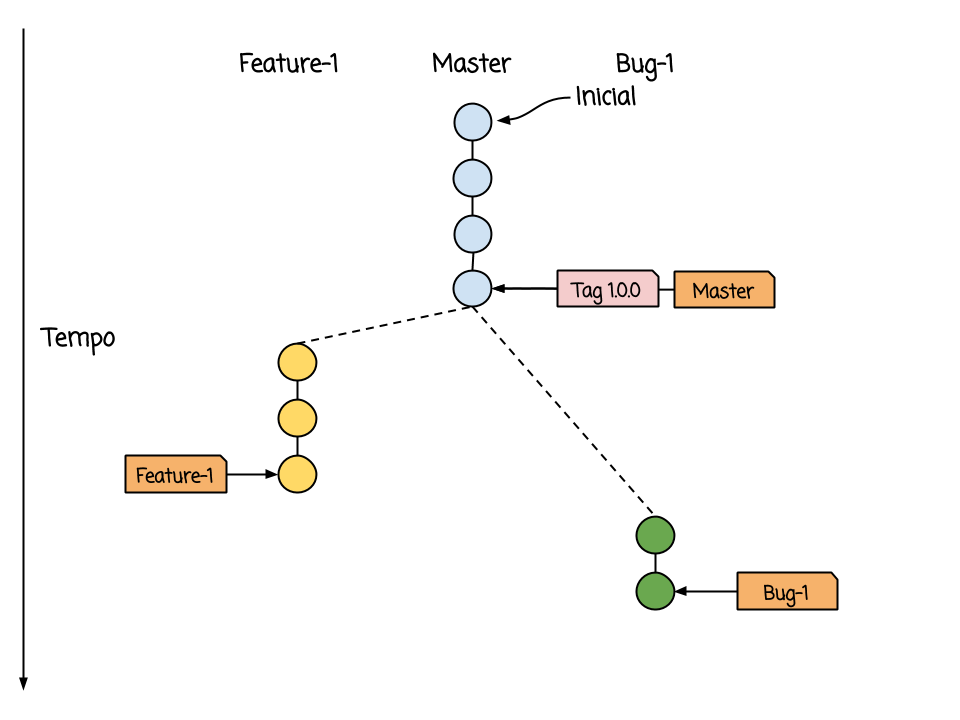
\includegraphics[width=1\textwidth]{img/proposal-01}
\end{figure}
}

\frame{\frametitle{Proposta de Processo de Trabalho (parte 2)} 
\begin{figure}[h!]
\centering
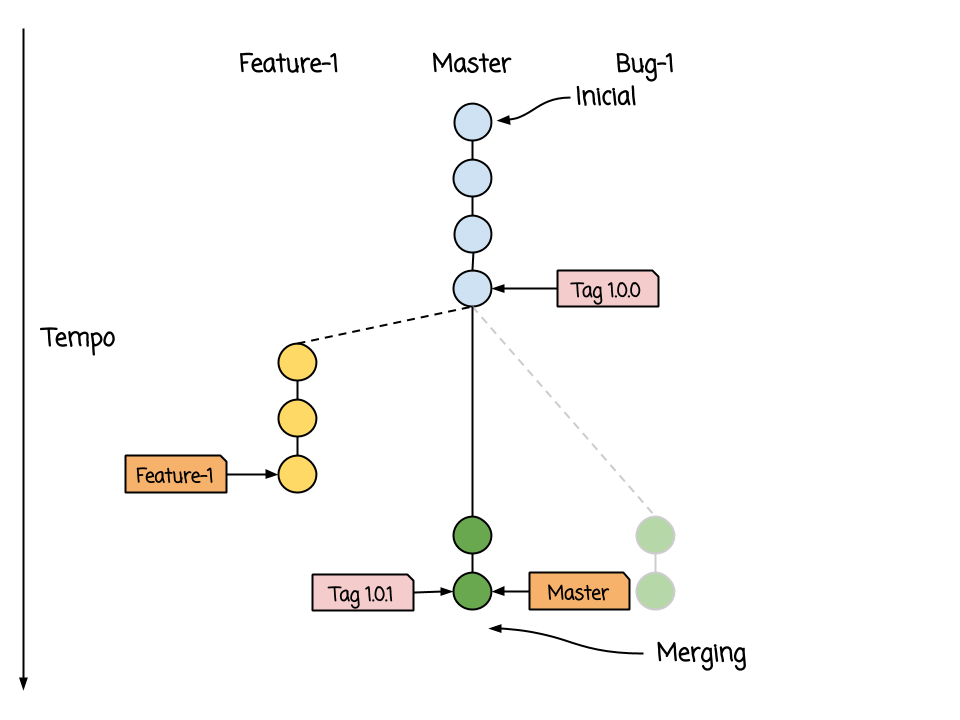
\includegraphics[width=1\textwidth]{img/proposal-02}
\end{figure}
}

\frame{\frametitle{Proposta de Processo de Trabalho (parte 3)} 
\begin{figure}[h!]
\centering
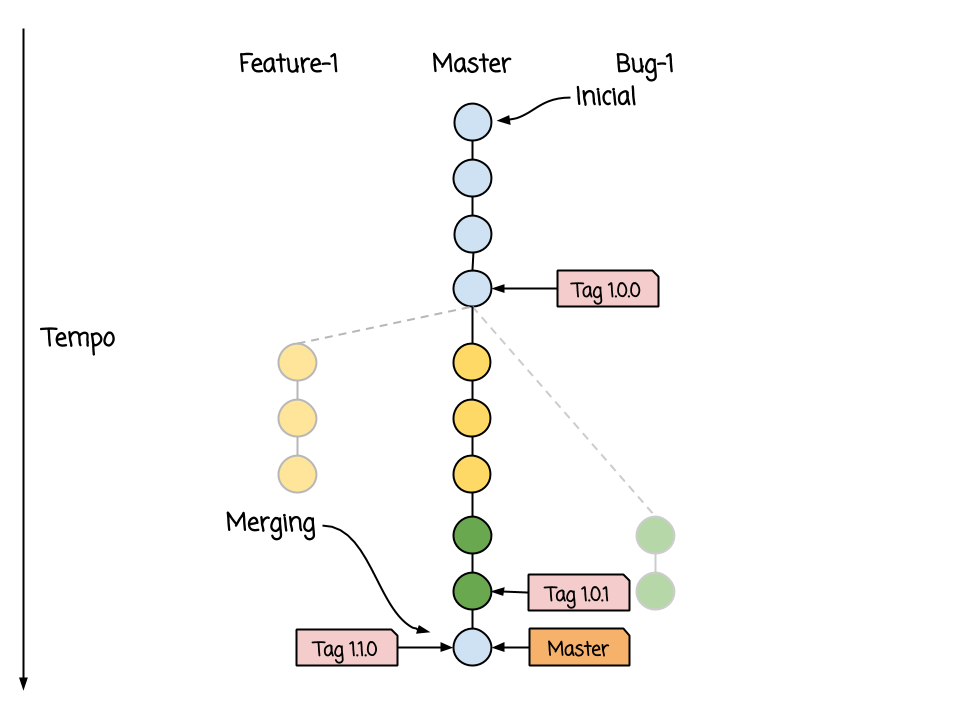
\includegraphics[width=1\textwidth]{img/proposal-03}
\end{figure}
}

\frame{\frametitle{Proposta de Processo de Trabalho (parte 3)} 
\begin{figure}[h!]
\centering
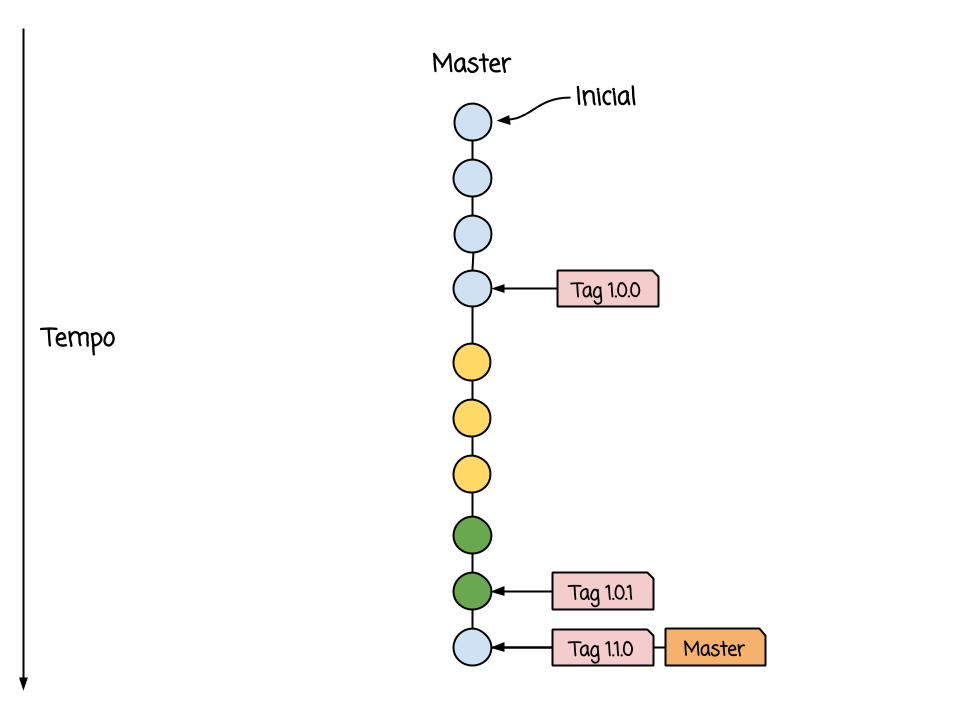
\includegraphics[width=1\textwidth]{img/proposal-04}
\end{figure}
}

\section{Alterações ao Esquema de Banco do Cube} 

\frame{ 
\begin{figure}[h!]
\centering
{\fontsize{1cm}{1em}\selectfont Esquema de banco do Cube}
\end{figure}
}

\frame{\frametitle{Contratempos} 
    \begin{itemize}
        \item perdemos o processo que tinhamos para atualizacao do esquema de
            banco do Cube;
        \newline
        \item dificuldade para criar ou manter ambientes de desenvolvimento
            atualizados;
        \newline
        \item contratempos e sobrecarga da equipe de BD.
    \end{itemize}
}

\frame{\frametitle{Proposta} 
    \begin{itemize}
        \item criar um repositorio para abrigar os \textit{scripts} do Cube.
            Facilitando o compartilhamento das alteracoes;
        \newline
        \item definir um processo de trabalho para manutencao dos
            \textit{scripts}. Colaboracao entre equipes de Desenv e BD.
    \end{itemize}
}

\frame{\frametitle{Proposta de Fluxo de Trabalho} 
\begin{figure}[h!]
\centering
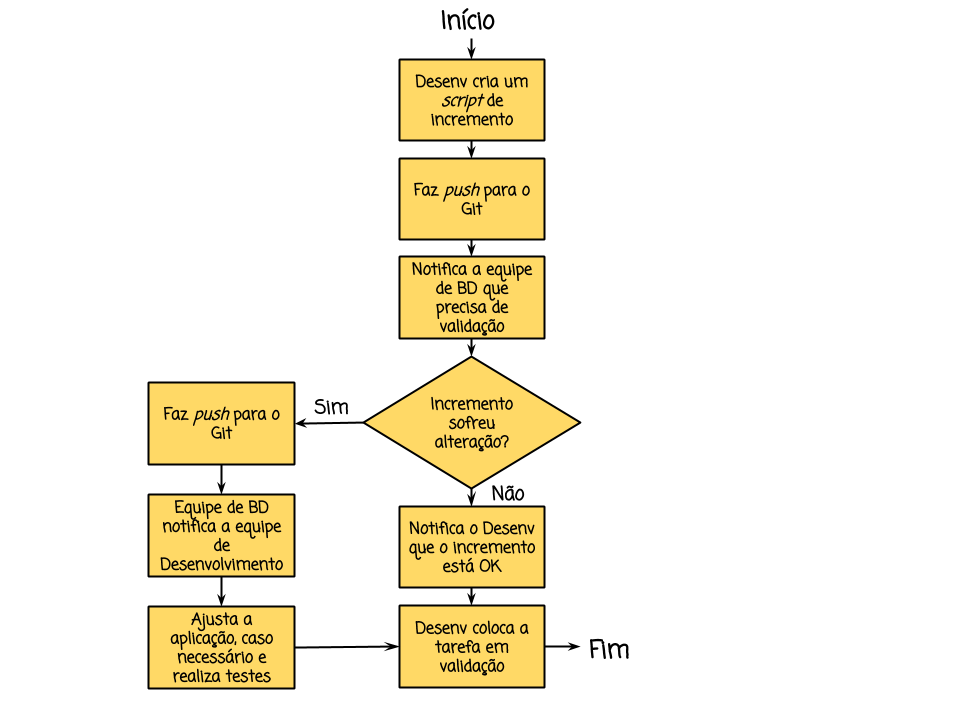
\includegraphics[width=1\textwidth]{img/fluxo}
\end{figure}
}

\frame{ 
\begin{figure}[h!]
\centering
{\fontsize{2cm}{1em}\selectfont Obrigado!}
\end{figure}
}
\end{document}

